\documentclass{atistandalonetask}
\usepackage{atistandard}

\begin{document}
  \begin{atiTask}[
    title = Integralsatz
  ]

Gegeben sei das Vektorfeld 
\[\vec{F}=\vec{r}\times (\vec{i}+\vec{j}+\vec{k}).\] Es sei $C$ der Weg, der durch den Schnitt zwischen dem Rotationsellipsoid $2(x^2+y^2)+z^2=1$ und der Ebene $z=1/\sqrt{2}$ gegeben ist.  Berechnen Sie die Zirkulation 
\[\oint _C\vec{F}\D\vec{r}
\]
	\begin{atiSubtasks}
		\item direkt aus dem Wegintegral
		\item nach Anwendung eines Integralsatzes als Oberflächenintegral.
	\end{atiSubtasks} 
	Fertigen Sie eine Skizze des Integrationsgebietes an.
  \end{atiTask}
  \begin{atiSolution}
  Lösung folgt
   %   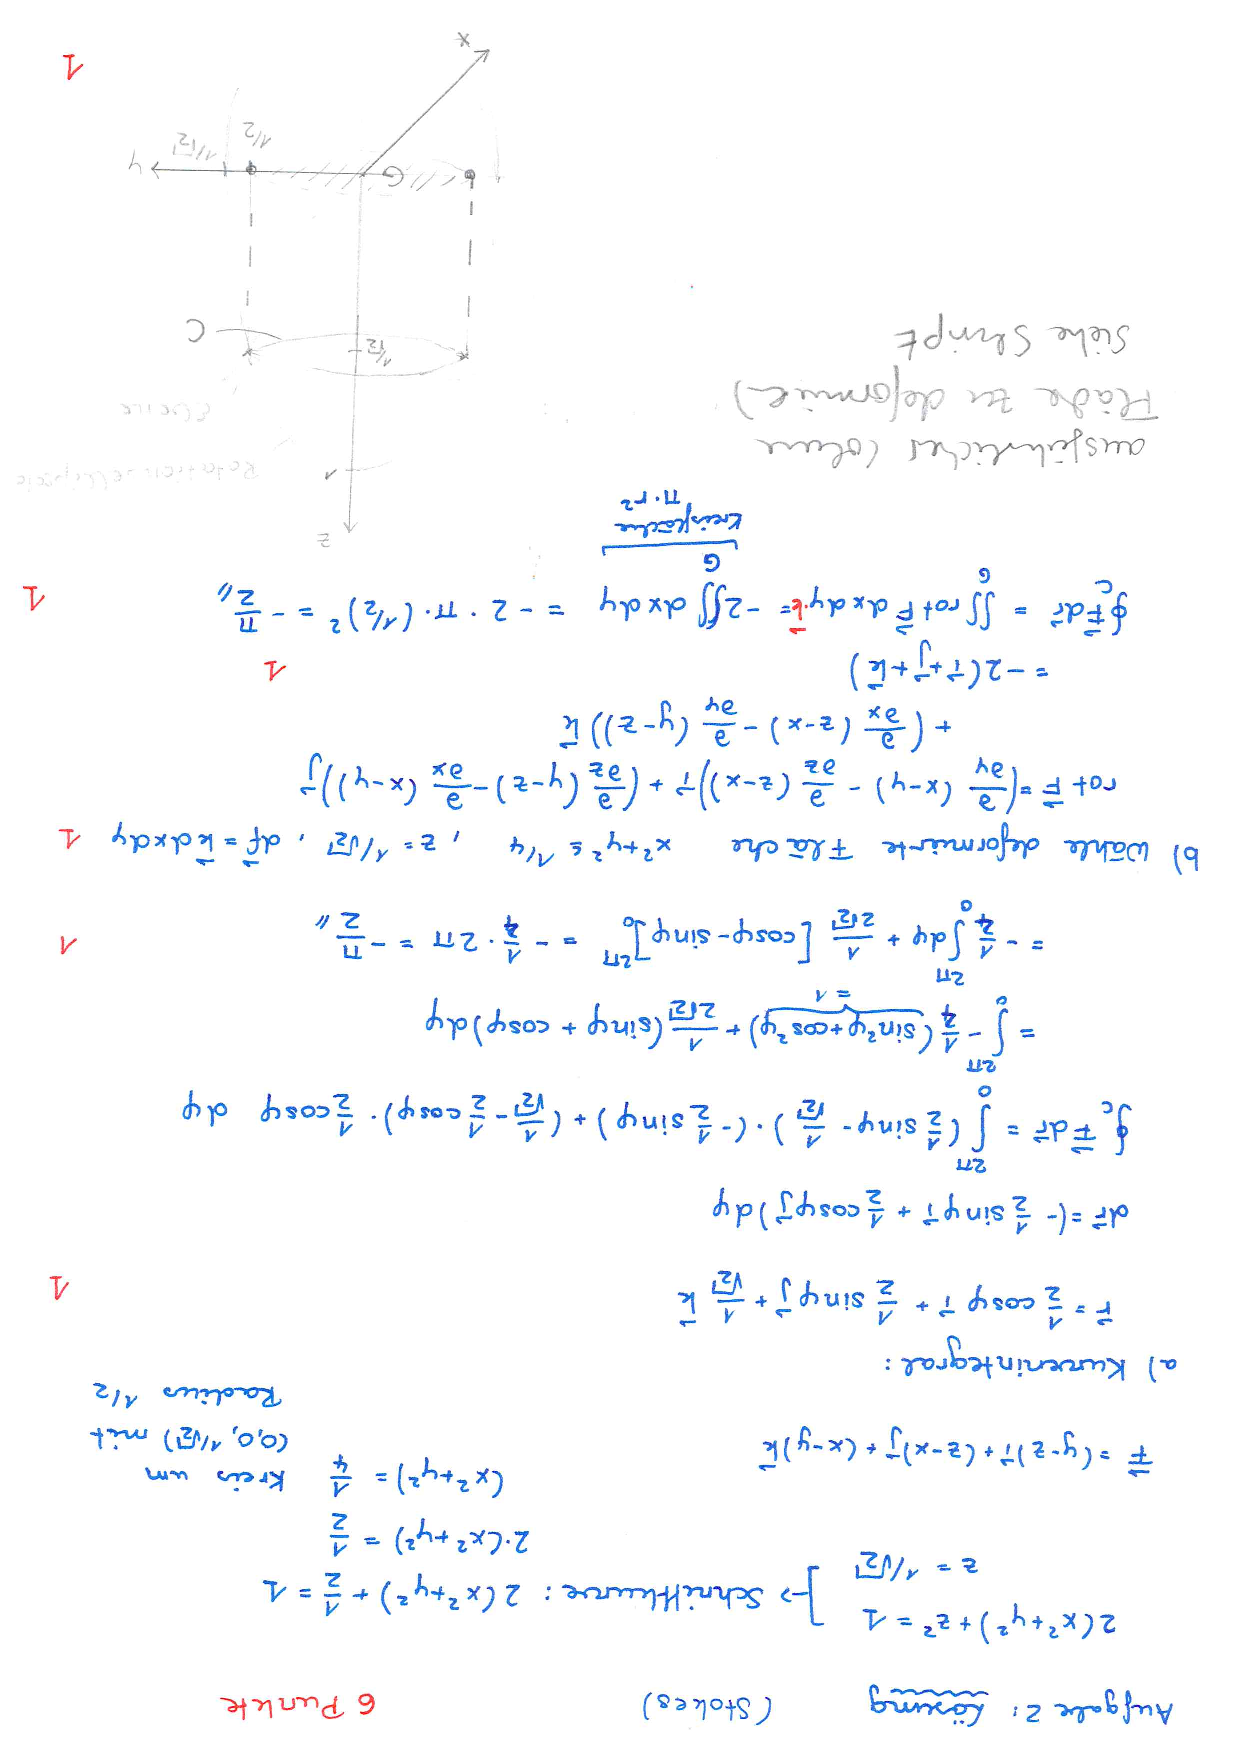
\includepdf[pages=-]{solution-stokes_vi.pdf}
  \end{atiSolution}
\end{document}